\documentclass[border=10pt]{standalone}
\usepackage{tikz}\usepackage{amsmath}\usetikzlibrary{arrows.meta}
\begin{document}
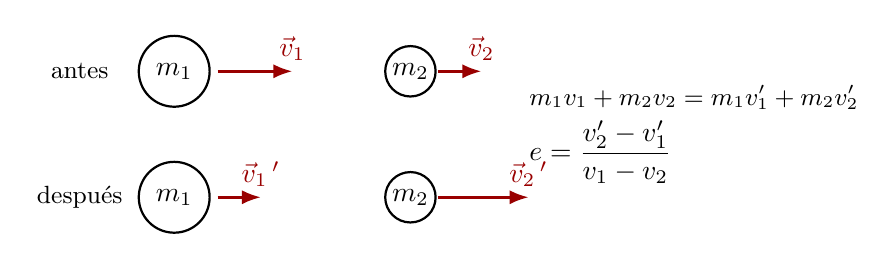
\begin{tikzpicture}[line width=0.9pt,>={Latex[length=2.4mm]}]
  % antes
  \node at (-1.2,1.4){\small antes};
  \draw[thick] (0,1.4) circle(0.45) node{$m_1$};
  \draw[thick] (3,1.4) circle(0.32) node{$m_2$};
  \draw[->,red!60!black] (0.55,1.4)--(1.5,1.4) node[above]{$\vec v_1$};
  \draw[->,red!60!black] (3.35,1.4)--(3.9,1.4) node[above]{$\vec v_2$};
  % despues
  \node at (-1.2,-0.2){\small después};
  \draw[thick] (0,-0.2) circle(0.45) node{$m_1$};
  \draw[thick] (3,-0.2) circle(0.32) node{$m_2$};
  \draw[->,red!60!black] (0.55,-0.2)--(1.1,-0.2) node[above]{$\vec v_1\,'$};
  \draw[->,red!60!black] (3.35,-0.2)--(4.5,-0.2) node[above]{$\vec v_2\,'$};
  \node[align=left] at (6.6,0.6){\small $m_1v_1+m_2v_2=m_1v_1'+m_2v_2'$\\[3pt]$e=\dfrac{v_2'-v_1'}{v_1-v_2}$};
\end{tikzpicture}
\end{document}
